%%%%%%%% ICML 2021 EXAMPLE LATEX SUBMISSION FILE %%%%%%%%%%%%%%%%%

\documentclass{article}

% Recommended, but optional, packages for figures and better typesetting:
\usepackage{microtype}
\usepackage{graphicx}
\usepackage{subfigure}
\usepackage{booktabs} % for professional tables

% hyperref makes hyperlinks in the resulting PDF.
% If your build breaks (sometimes temporarily if a hyperlink spans a page)
% please comment out the following usepackage line and replace
% \usepackage{icml2021} with \usepackage[nohyperref]{icml2021} above.
\usepackage{hyperref}
\usepackage{float}

\usepackage{xurl}
\setlength{\textfloatsep}{10pt plus 1.0pt minus 2.0pt}
\setlength{\floatsep}{10pt plus 1.0pt minus 2.0pt}
\setlength{\intextsep}{10pt plus 1.0pt minus 2.0pt}

% Attempt to make hyperref and algorithmic work together better:
\newcommand{\theHalgorithm}{\arabic{algorithm}}

% Use the following line for the initial blind version submitted for review:
%\usepackage{icml2021}

% If accepted, instead use the following line for the camera-ready submission:
\usepackage[accepted]{icml2021}

% The \icmltitle you define below is probably too long as a header.
% Therefore, a short form for the running title is supplied here:
\icmltitlerunning{Image Recognition and Joint Detection for Rock Paper Scissors}

\begin{document}

\twocolumn[
\icmltitle{Image Recognition and Joint Detection for Rock Paper Scissors\\
CS 4262/5262 Foundations of Machine Learning Spring 2024\\ ML Mavericks Graduate Project}

% It is OKAY to include author information, even for blind
% submissions: the style file will automatically remove it for you
% unless you've provided the [accepted] option to the icml2021
% package.

% List of affiliations: The first argument should be a (short)
% identifier you will use later to specify author affiliations
% Academic affiliations should list Department, University, City, Region, Country
% Industry affiliations should list Company, City, Region, Country

% You can specify symbols, otherwise they are numbered in order.
% Ideally, you should not use this facility. Affiliations will be numbered
% in order of appearance and this is the preferred way.
\icmlsetsymbol{equal}{*}

\begin{icmlauthorlist}
\icmlauthor{Marcus Kamen}{to}
\icmlauthor{Xutao Mao}{to}
\icmlauthor{Galen Wei}{to}
\icmlauthor{Joseph Zou}{to}
\end{icmlauthorlist}

\icmlaffiliation{to}{CS 4262/5262, Department of Computer Science, Vanderbilt University, Nashville, Tennessee, United States}

\icmlcorrespondingauthor{}{marcus.p.kamen@vanderbilt.edu}
\icmlcorrespondingauthor{}{xutao.mao@vanderbilt.edu}
\icmlcorrespondingauthor{}{galen.wei@vanderbilt.edu}
\icmlcorrespondingauthor{}{joseph.a.zou@vanderbilt.edu}

% You may provide any keywords that you
% find helpful for describing your paper; these are used to populate
% the "keywords" metadata in the PDF but will not be shown in the document
\icmlkeywords{Machine Learning, ICML}

\vskip 0.3in
]

% this must go after the closing bracket ] following \twocolumn[ ...

% This command actually creates the footnote in the first column
% listing the affiliations and the copyright notice.
% The command takes one argument, which is text to display at the start of the footnote.
% The \icmlEqualContribution command is standard text for equal contribution.
% Remove it (just {}) if you do not need this facility.

\printAffiliationsAndNotice{}  % leave blank if no need to mention equal contribution
%\printAffiliationsAndNotice{\icmlEqualContribution} % otherwise use the standard text.

\begin{abstract}
For this paper, we investigated image recognition of rock paper scissors hand gestures, using both the images directly and joint detection on the images. We used a Base dataset, including only hands on a white background, and an Expanded dataset, including hands on different backgrounds and non-hand images. We also ran both datasets through joint detection to augment them with landmarks. We found that joint detection improved the accuracy of models from prior research and allowed us to improve robustness through our Expanded dataset. Using joint detection, we created a game playing program for live images.
\end{abstract}

\section{Introduction}
\label{submission}

Rock Paper Scissors is a popular two-player game in which players choose between rock, paper, and scissors, and show their opponent their hand shaped as their choice. For humans, it is very easy to recognize the difference between these choices in a game. However, if a computer plays against a human or if two humans play and the computer watches, the computer must include image recognition to understand what the human has chosen for their hand position. The goal of this paper is to examine different methods of rock paper scissors image recognition, allowing for the creation of a game playing program for games against either a computer or another person.\\
Although rock paper scissors game playing itself may have limited use cases, our findings can be applied to hand gesture recognition in general, which has many important uses.
For example, previous research has been conducted on hand gesture recognition for human sign language. In one such study, the researchers used a convolutional neural network to recognize sign language. However, this study only reached validation accuracy of 60\%, indicating that more research can be done to improve the accuracy of hand gesture recognition models \cite{Chowdary2023SignLR}. In addition, we believe that creating a game playing program is essential to the importance of our results. For our models to be used, for rock paper scissors or any other similar task, a computer would need to be set up to recognize images in real time. Similar programs have been created in the past, but we believe that we can improve these programs by improving the underlying classification models to run the program and extending the datasets used \cite{Aphiratsakun2020AIbasedRP}. \\
Previous studies have already been conducted on rock paper scissor image recognition. For example, one such study has been conducted on the efficacy of Convolutional Neural Networks (CNNs) for a rock paper scissors image dataset from Kaggle \cite{kaggle}. This study reached 99\% test accuracy on relevant datasets \cite{CNNM}. In addition, another study has used a pre-trained image recognition model called AlexNet to employ transfer learning to the problem, reaching 99.54\% test accuracy on the same dataset \cite{Ahmed2023RockPaperScissorsIC}. However, neither study attempts a feature reduction technique which may decrease training time. Furthermore, the two studies maintain the background and coloration of the original image. However, Chen et al. shows that eliminating background noise, skin color, and other unnecessary information in the images to produce a black and white is a simple but effective scheme for classification \cite{Chen2010RockPA}. Finally, these studies were both conducted on the same Kaggle dataset, only with pictures of the same background and image direction, all constituting one of rock, paper, or scissors. However, to simulate a live game-playing environment, it is necessary to include negative data (images with no hands), diverse backgrounds, and diverse hand positions. To this end, we incorporate multiple datasets, ensuring that our models can detect rock paper scissors images in different positions and determine if an image does not have a relevant hand present.\\
In addition, other machine learning methods have garnered success but have not been used on rock paper scissors images. For example, Support Vector Machines (SVMs) can be used for classification problems with more than two classes for image recognition. Likewise, the Vision Transformer (ViT) is a relatively new architecture that has seen success in image classification \cite{vit}. Therefore, we will test our models with SVMs and ViT.\\
Unlike previous work, we incorporate joint detection for rock paper scissor image recognition. Our hypothesis is that the joints of the human hand are the most important aspect of rock paper scissors images because joints can be used to easily infer overall hand position. Therefore, detecting joints and then running classification models on the results could produce more accurate results. Our goal is to create joint landmarks for all images, then run models on the joint landmarks. MediaPipe, an open source framework for image detection, has already been proven useful in joint detection tasks for the whole body, proving its general efficacy \cite{9973559}. In addition, MediaPipe has previously been used on hand joints, providing over 85\% precision \cite{DBLP:journals/corr/abs-2006-10214}. Also, MediaPipe has previously been used for detecting hands in sign language, a more complex task than 3-way classification, producing up to 99\% accuracy \cite{kavana2022recognization}. Therefore, MediaPipe has been proven for other image classification tasks, so we will attempt to extend these models to rock paper scissors. \\
Our goal is to use joint detection as an intermediary in our machine learning model. So, we will run images through joint detection models, generate the landmark results, and then run those results through more machine learning models for rock paper scissors image classification. This method of using joint detection has been used on similar tasks. One study used similar models to detect landmarks on faces and then use those landmarks to predict facial expressions, producing up to 99.24\% accuracy, comparable with other types of facial expression recognition methods \cite{8528894}.\\
K-means clustering may also produce strong accuracy on the datasets. K-means clustering is usually helpful when correct labels are not available, forcing unsupervised learning to be used. However, we hypothesize that, when comparing the labels produced by k-means clustering with three centroids to the actual labels of the data, we will find that the produced labels are very similar, indicating that k-means clustering can be used to classify the data. Although this is an unorthodox approach to using k-means clustering, k-means clustering has been studied in this way before on already labeled data for Breast Cancer and Diabetes \cite{10.1007/978-3-642-14834-7_40}.\\
In total, our goal is to expand upon previous research in rock paper scissors image recognition by creating new models such as SVMs and k-means clustering, expanding the dataset to include negative data, using joint detection to enhance the data prior to classification, and using our findings to create a game playing program.

\section{Methods} 

\subsection{Datasets}
We used two datasets: Base and Expanded. The Base dataset contains only rock paper scissors images, all from one source. The Expanded dataset contains images from multiple sources, including images not constituting rock, paper, or scissors. The Expanded dataset helps improve robustness and generalizability. \\
The Base dataset was extracted from Hugging Face, and consists of artificially generated hand images on a white background \cite{Moroney}. The images are 300 $\times$ 300 pixels \cite{huggingface}, with an even split between rock, paper, and scissors images. \\
The Expanded dataset has three parts. The first part is the Base dataset. The second part is the same dataset from Kaggle used in previous research into rock paper scissors image recognition \cite{kaggle}. This dataset consists of 300 $\times$ 200 pixel images of real hands on a green background, also evenly split among each category. The third part is a dataset of background images that constitute none of rock, paper, or scissors. These background images were extracted from a set of stock background images originally introduced in an article on image matting \cite{stock} \cite{stockarticle}. We uploaded the Expanded dataset to Hugging Face at 
\url{https://huggingface.co/datasets/conjunct/rps_annotated}. \\
The Base dataset's existing train/test split is used, while the Kaggle and BG-20k datasets have a train/test split of 75\%/25\%. The Base dataset has an overall 87.1\%/12.9\% train/test split, while the Expanded dataset is split 81.8\%/18.2\%.

\begin{table}[h]
\vskip -0.15in
\caption{Dataset Information}
\label{tab:data_sets}
\centering
\small
\begin{tabular}{c | c | c | c}
\toprule
Dataset & Creator & Train Count & Test Count \\
\midrule
Base & Moroney, Laurence & 2520 & 372 \\
\midrule
Kaggle & DRGFREEMAN & 1750 & 438 \\
\midrule
BG-20k & Li et al. & 4900 & 1225 \\
\midrule
Expanded & Combined & 9170 & 2035 \\
\bottomrule
\end{tabular}
\vskip -0.1in
\end{table}

\subsection{Preprocessing}

To ensure that images were in a consistent format, we resized all of images to a size of 256 $\times$ 256, or 65536 pixels. Then, we randomly horizontally and vertically flipped the images to minimize effects from image orientation. Finally, we grayscaled the image to remove the effect of color on the images, reducing the images to 1 channel (black/white) instead of 4 (red, blue, green, alpha). \\
Next, we reduced features in two different ways. Since the images have 65536 pixels and there are only 2520 images total in the Base set, feature reduction is needed to limit overfitting and reduce training time. \\
To this end, we first ran Principal Components Analysis (PCA) on the base dataset. We ran PCA on the default number of components by Scikit-Learn, which is equivalent to the number of images. We then plotted amount of explained variance with respect to the number of components. Our result is in Figure 1. Fewer than 3000 components explain \textgreater 99.9\% of the variance in the data, reducing the dimensionality 21-fold $(65536 \rightarrow 3000)$. To decide the minimum number of components necessary, we tested different amounts of variance explained on different numbers of components and compared model train time and model accuracy. This process is further discussed in Section 3.1. \\
In addition to PCA, our second method of feature reduction was joint detection. Joint detection was conducted on both the Base and Expanded datasets. In order to process our data through joint detection, we used Google's MediaPipe for augmenting the images with landmarks. The landmarks contain the x, y, and z coordinates of different points on each hand, allowing for easy tracking of hand gestures. Figure 2 shows one image and its augmented landmarks.

\begin{figure}[h]
\begin{center}
\centerline{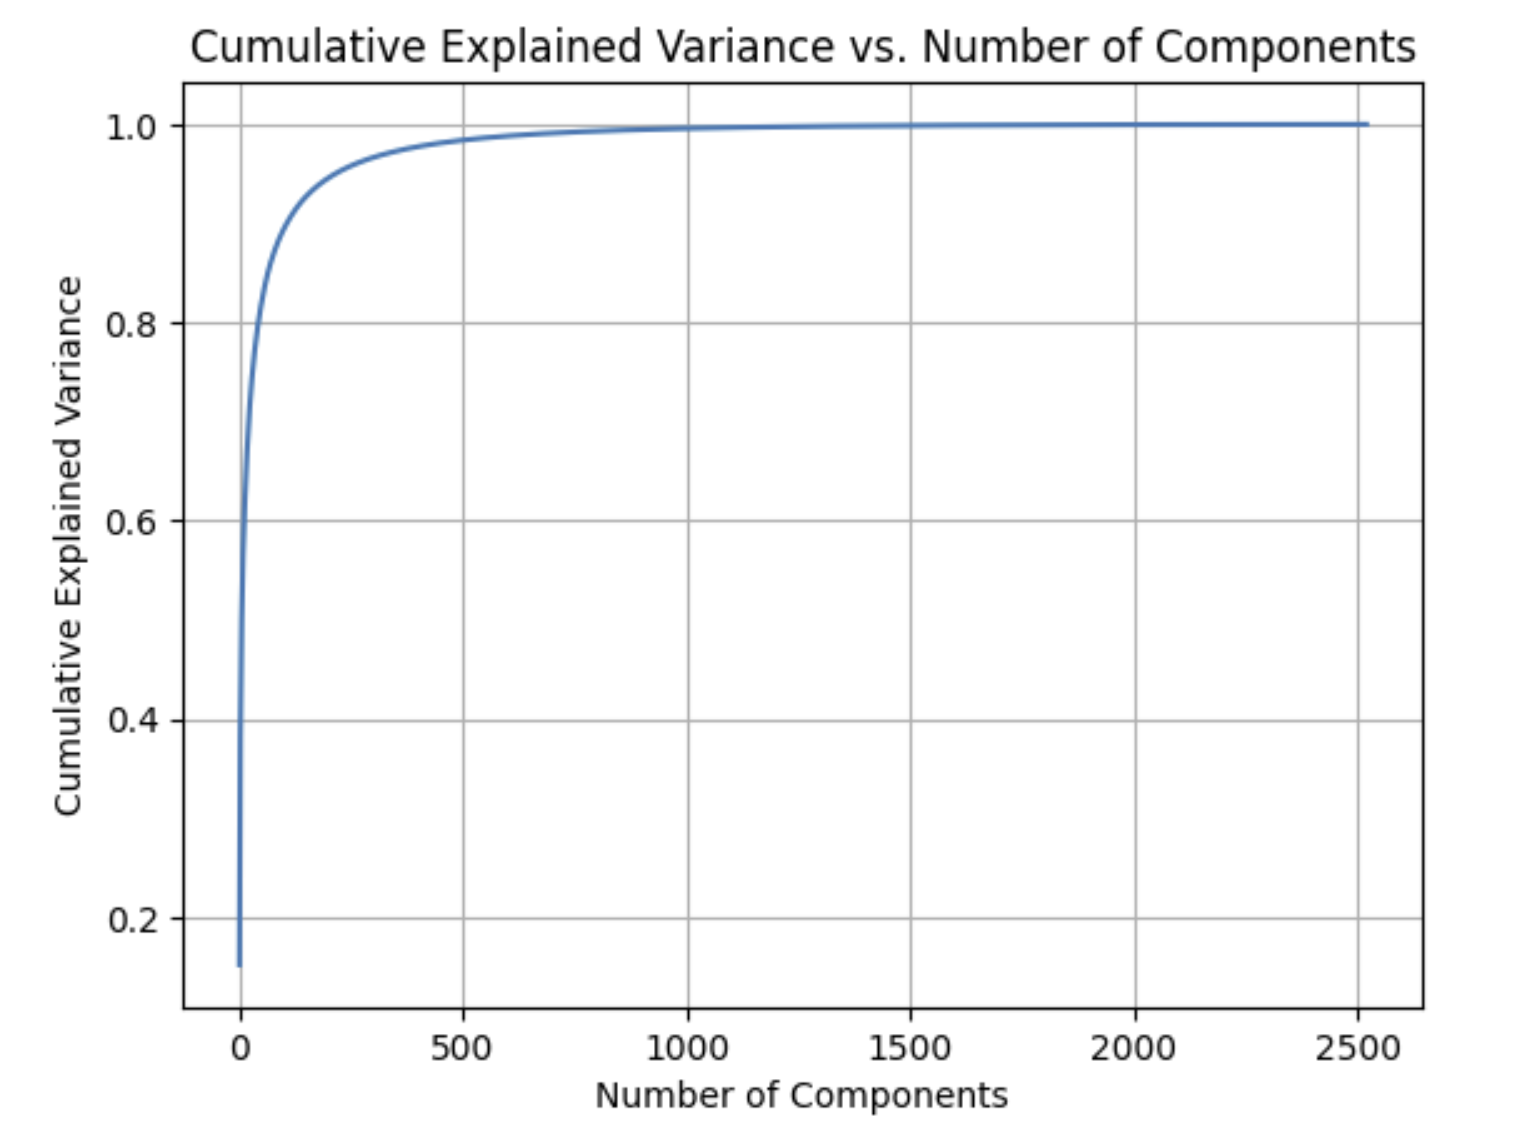
\includegraphics[width=\columnwidth]{variance_explained_base.png}}
\caption{Variance Explained by Number of Components for Base Dataset}
\end{center}
\begin{center}
\centerline{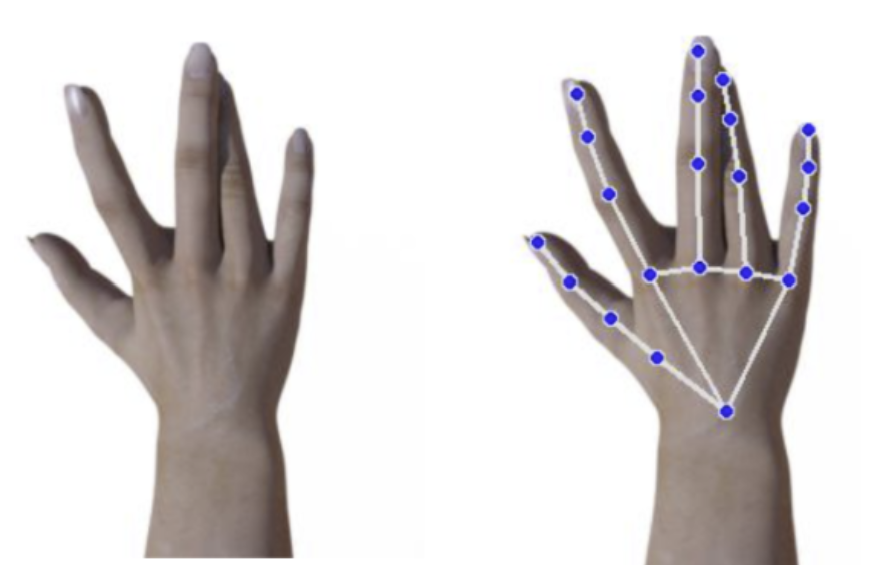
\includegraphics[width=\columnwidth]{joint_augment.png}}
\caption{Joint Landmarks Augmented on Example Image}
\end{center}
\vskip -0.1in
\end{figure}

\subsection{Machine Learning Approaches}
We ran many machine learning algorithms on both the Base and Expanded datasets. The goal of these algorithms is to classify between rock, paper, and scissors (or "none", for the Expanded dataset) with maximum accuracy. We chose accuracy as our most important metric. Since our datasets were evenly split between all categories, accuracy is a balanced metric for determining if our models correctly classify the data. We collected F1-scores when available to ensure that our accuracy was not skewed by the number of images in each class, especially for the negative data in the Expanded dataset. Confusion matrices were also collected to identify common misclassifications. Base models were evaluated with the Base test set, while Expanded models were evaluated with the Expanded test set. \\
First, we ran Support Vector Machine (SVM) models on varying numbers of PCA components to compare their performance based on model train time and model accuracy. Then, we chose the best combination of these factors to decide how many components was best for the PCA. We used the radial basis function for our SVM kernel. Next, we ran a Convolutional Neural Network on both the Base and Expanded datasets. We adapted the existing DenseNet161 architecture \cite{densenet}. By using a model pre-trained on ImageNet-1k, a dataset of 1000 different image classes, we can use transfer learning to fine tune the model on our specific datasets. Finally, we fine-tuned a pretrained ViT-B/16 on the Expanded dataset \cite{vit}. \\
For joint detection preprocessed data, we ran three models on the base dataset and three models on the Expanded dataset. For the base dataset, we ran an SVM using the linear kernel, k-means clustering, and a Neural Network with Adam optimizer, cross entropy loss function, and 3 layers of 64, 64, and 3 neurons respectively, using the ReLU activation function. For our Expanded dataset, we ran k-means clustering and two different SVM models with the radial basis function kernel, one including all joints and one including just the distances to the fingers from the wrist. Note that all other joint detection based models, only excluding the one version of the SVM model, use only distances to the fingers from the wrist. We decided to only use this data from our knowledge of rock, paper, and scissors hand positions. For paper, all fingers should be far away from the wrist. For scissors, the pointer and middle fingers should be far away from the wrist, while the other fingers should be close to the wrist. For rock, all fingers should be close to the wrist. Therefore, the distances from the wrist to the fingers are the most important features, so adding other features may produce overfitting. \\
The Media Pipe joint detection model will not augment landmarks to images it does not think are hands. This gives us an easy way to classify the images that do not consist of rock, paper, or scissors. Note that about 7\% of the images in the Kaggle dataset do not have joint detection landmarks augmented since the hands are not completely in frame. We ignore these images as they are not completely visible to the computer, so they do not give as much data for classification. Since our goal is to create a game playing program, we can assume that the user will always put their hand in frame. \\
We also attempted some models that we will not be discussing thoroughly in this paper. We chose not to discuss them due to various constraints such as accuracy and importance of results. These models include Neural Networks on PCA Base dataset, SVMs and NNs on PCA Expanded dataset, and different variations of using joint detection landmarks for SVMs and NNs on both datasets.

\subsection{Game Playing Program}
In addition to creating models for image recognition, we implemented a game playing program to test if our models could be used by a computer and human to actually play rock paper scissors. To implement the program, we used OpenCV, a computer vision library for real time computer vision. Our goal was to create a program that could allow users to place their hands in front of the camera, see joint detection landmarks in real time, and see the classification by our program. This could allow the user to actually play rock paper scissors using computer vision, either against the computer or against another human player. Either the SVM or NN on the Base dataset can be used as the underlying classification model for this game playing program . Once the program detected a hand, the joint landmarks were created, and our SVM or NN model classifies based on the joint landmarks.

\section{Results}
The following subsections describe our results for each model that we ran. Note that for the figures, 0 is the label for paper, 1 is the label for rock, 2 is the label for scissors, and 3 is the label for none of the three hand positions. Unless otherwise noted, the models all took trivially little time to train after the preprocessing was completed.

\subsection{Support Vector Machines for PCA on Base Dataset}

After running PCA on the data, we ran SVMs on different amounts of components from PCA. We kept track of the amount of variance explained, number of components, time to train the SVM, and accuracy of the SVM. Our results are shown in Table 2. Note that it took 114 seconds to fit PCA to the maximum number of components. \\
The accuracies for these models are very low, in the range of 60\% validation accuracy, so SVM on PCA data is clearly not the correct way to classify the images with high accuracy. This is in spite of over 99.6\% accuracy on the training set for 90\% variance explained, and 99.96\% accuracy on the training set for 99.9\% variance explained.

\begin{table}[h]
\vskip -0.15in
\caption{SVM for PCA on Base Dataset}
\label{tab:pca_base}
\centering
\small
\begin{tabular}{p{1.5cm} | c | p{1.5cm} | c}
\toprule
Variance Explained & Components & SVM Train Time (s) & Accuracy \\
\midrule
90\% & 106 & 0.188 & 62.1\% \\
\midrule
95\% & 213 & 0.285 & 64.0\% \\
\midrule
97.5\% & 369 & 0.995 & 63.7\% \\
\midrule
99\% & 653 & 1.61 & 63.4\% \\
\midrule
99.9\% & 1580 & 2.59 & 63.2\%\\
\bottomrule
\end{tabular}
\vskip -0.1in
\end{table}

\subsection{Convolutional Neural Networks on Base Dataset using Images Directly}

As described before, we ran a CNN model on the Base dataset using transfer learning. We achieved 100\% validation accuracy on 5 epochs with 0.009 validation loss, much better than our SVM models. This model took about 5 minutes to train on a T4 GPU.

\subsection{Convolutional Neural Networks on Expanded Dataset using Images Directly}

We also ran a CNN (DenseNet161) model on the Expanded dataset using transfer learning. We achieved 99.85\% validation accuracy on 10 epochs with 0.008 validation loss. This model took about 20 minutes to train on a T4 GPU.

\subsection{Vision Transformers on Expanded Dataset using Images Directly}

We fine-tuned a pretrained ViT-B/16 on the Expanded dataset \cite{vit}. Our results are in Figure 3. We reached 99.56\% accuracy on the expanded test set on 3.48 epochs with 0.007 validation loss. This model took about 40 minutes to train on a T4 GPU.

\begin{figure}[h]
\begin{center}
\centerline{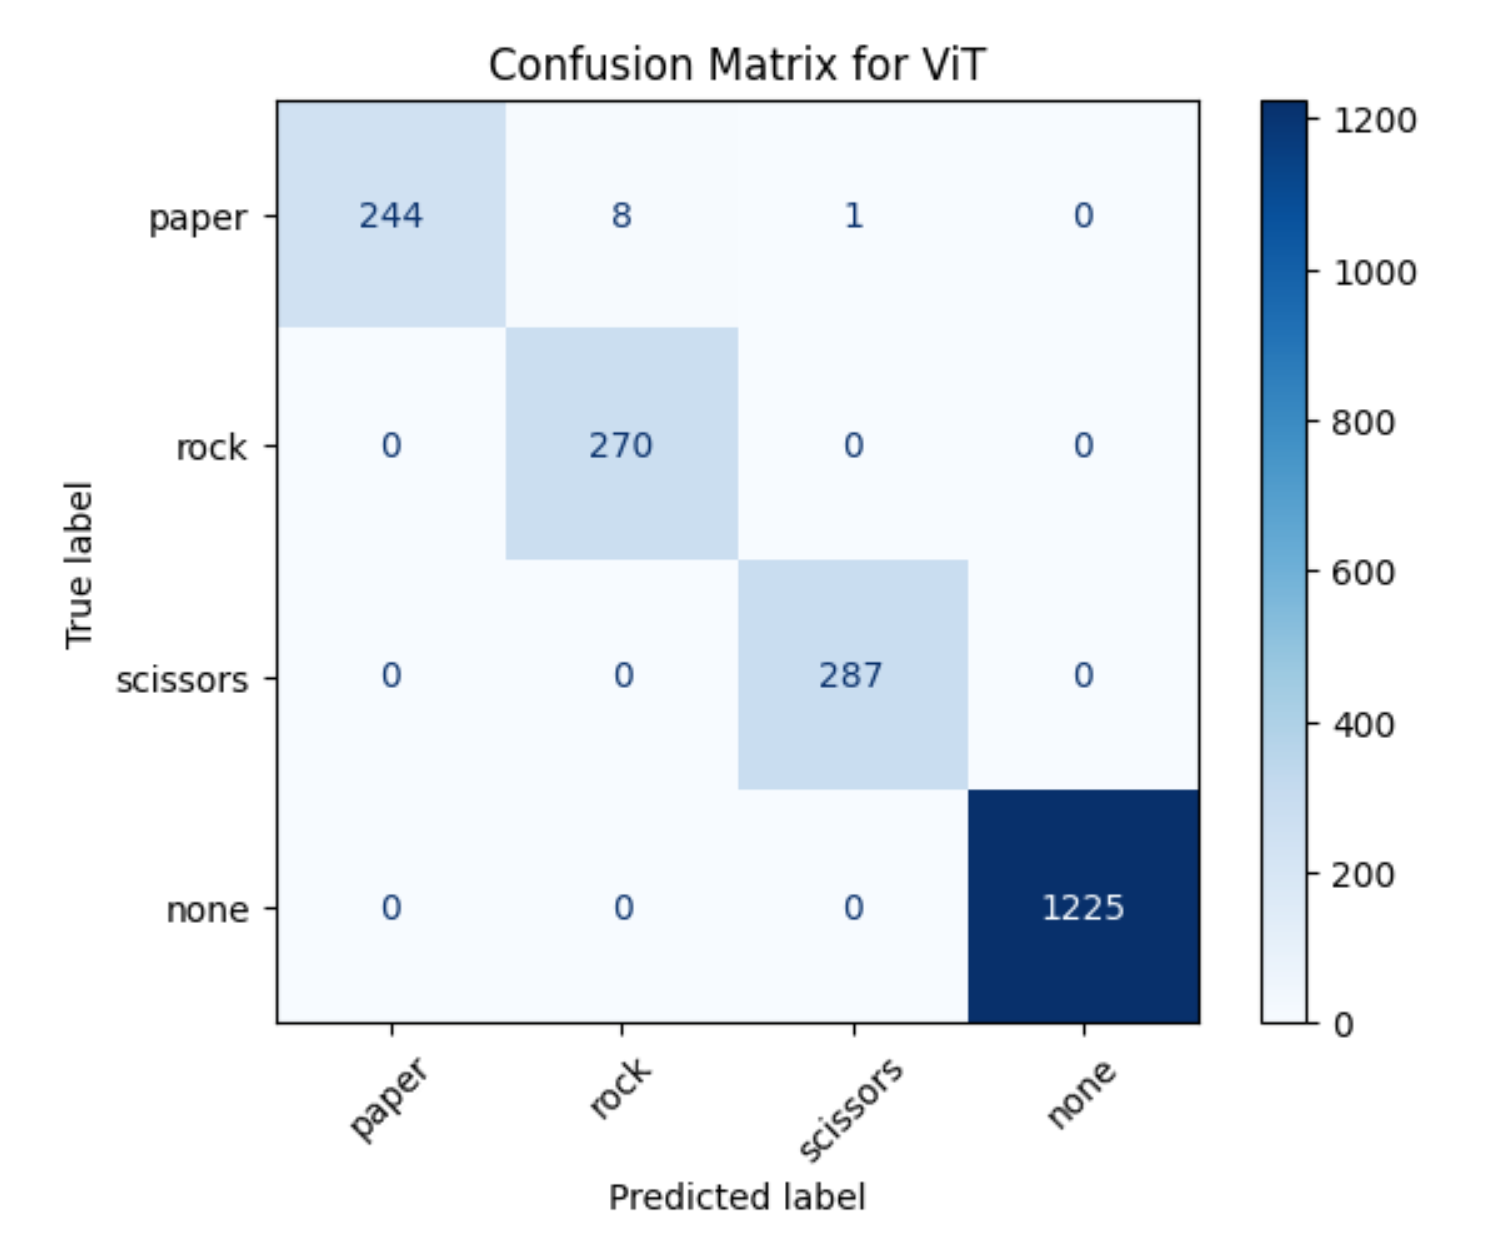
\includegraphics[width=\columnwidth]{vision_confus.png}}
\caption{Vision Transformer Confusion Matrix for Expanded Dataset}
\end{center}
\vskip -0.1in
\end{figure}

\subsection{Support Vector Machines for Joint Detection on Base Dataset}
As described previously, we ran SVMs on the joint detection data for the Base dataset. We reached perfect accuracy and F1-score for our model on our test set. Note that we also tested this model on a test set including both images from the Base dataset and Kaggle dataset, resulting in only one misclassification from rock to paper. Using this other test set, we show that our joint detection model is generalizable to other datasets.

\subsection{K-Means Clustering for Joint Detection on Base Dataset}
We ran k-means clustering for joint detection on the base dataset, and our metric for success was how accurately the created labels from k-means clustering represented the actual labels. We reached 80.2\% accuracy and 80\% F1-score. Our results are shown in Figure 4. Since this accuracy and F1-score is relatively low, k-means clustering was not particularly successful at classify the images of the Base dataset correctly.

\begin{figure}[h]
\begin{center}
\centerline{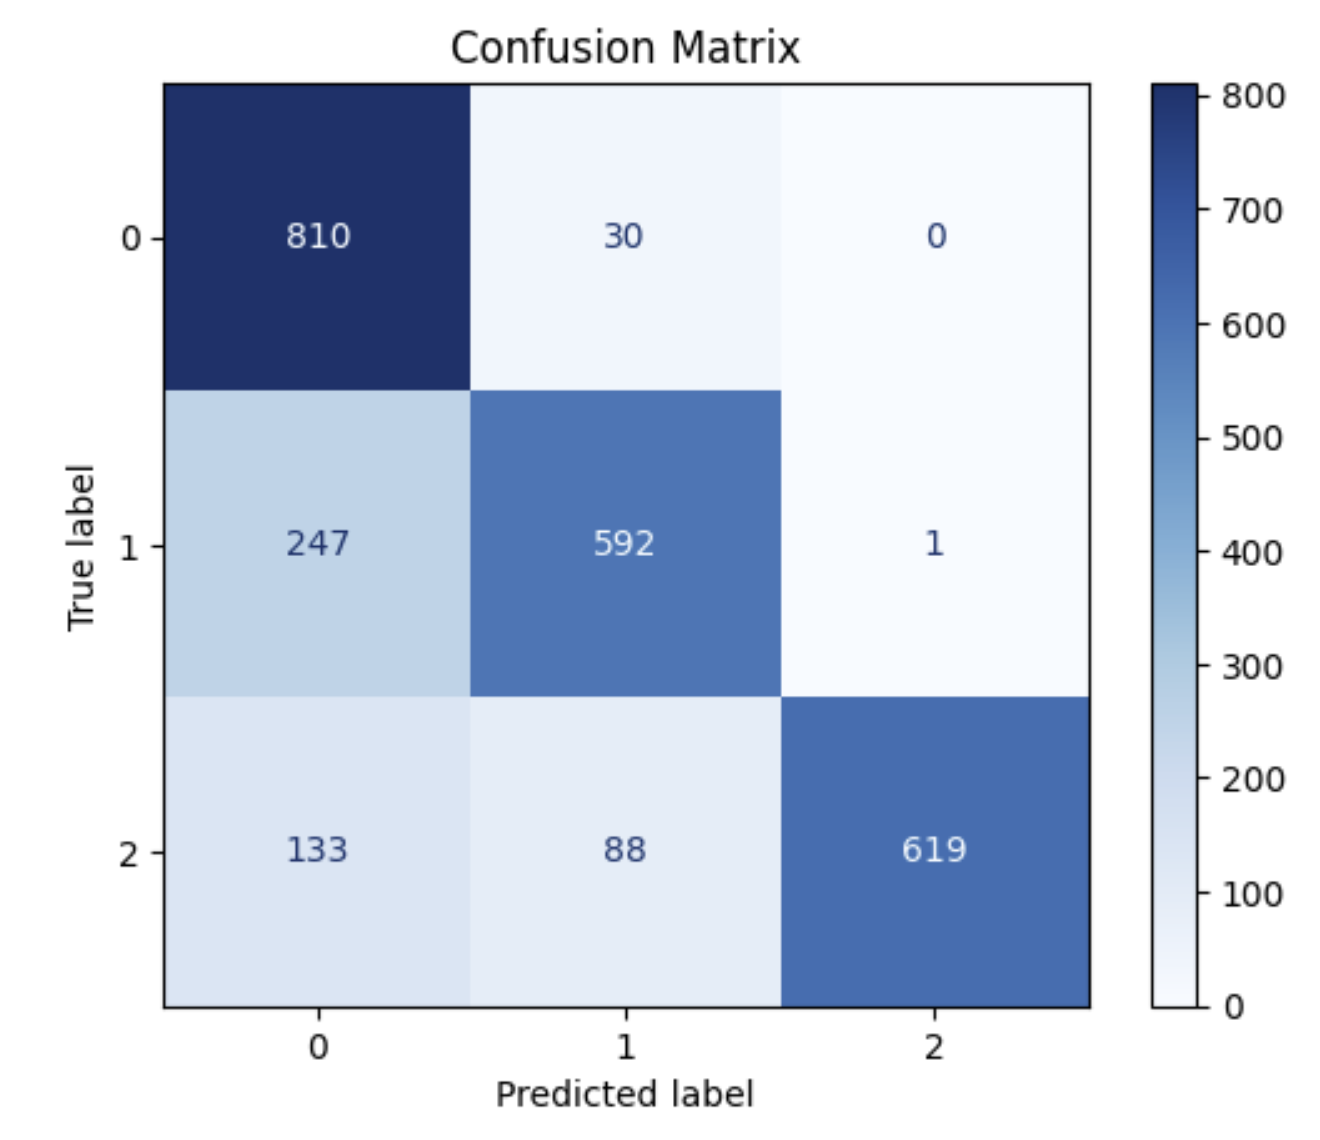
\includegraphics[width=\columnwidth]{kmeans_base_joint.png}}
\caption{K-means Clustering Confusion Matrix for Joint Detection on Base Dataset}
\end{center}
\end{figure}

\subsection{Neural Networks for Joint Detection on Base Dataset}
As described above, we ran a Neural Network on the joint detection data for the Base dataset. We reached perfect accuracy and F1-score for our model after 100 epochs on our test set. Note that we also tested this model on a test set including both images from the Base dataset and Kaggle dataset, also resulting in perfect accuracy. Using this other test set, we show that our joint detection model is generalizable to other datasets.

\subsection{K-Means Clustering for Joint Detection on Expanded Dataset}
We ran k-means clustering for joint detection on the Expanded dataset, and our metric for success was how accurately the created labels from k-means clustering represented the actual labels. We reached 86.8\% accuracy and 87\% F1-score. Our results are shown in Figure 5. Since this accuracy and F1-score is relatively low, k-means clustering was not particularly successful at classify the images of the Base dataset correctly.

\begin{figure}[h]
\begin{center}
\centerline{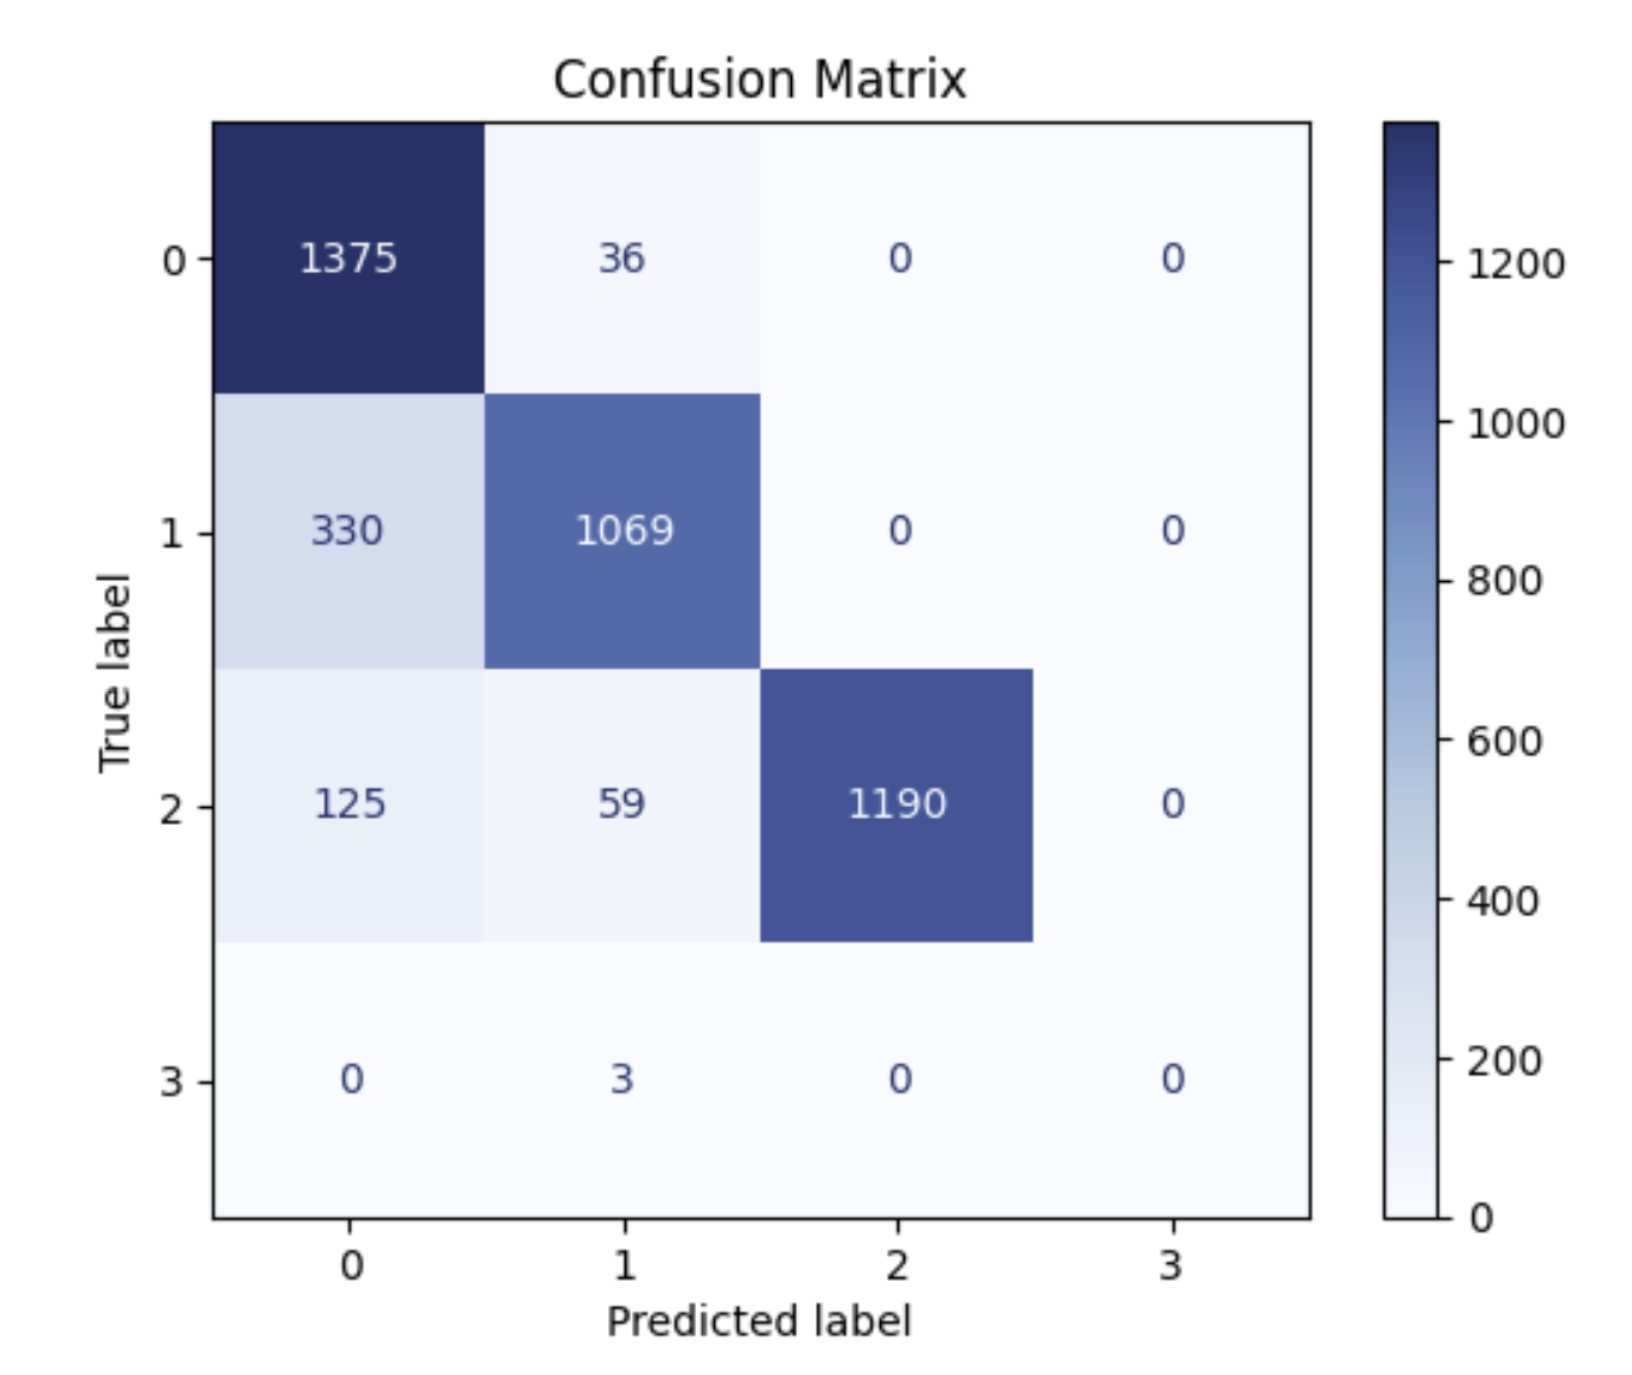
\includegraphics[width=\columnwidth]{kmeans_ex_joint.png}}
\caption{K-means Clustering Confusion Matrix for Joint Detection on Expanded Dataset}
\end{center}
\end{figure}

\subsection{Support Vector Machines for Joint Detection on Expanded Dataset With Distances from Wrist to Fingers}
As described previously, we ran a support vector machine model for joint detection on the Expanded dataset, only including the distances from the wrist to the fingers. Our results are in Figure 6. We reached 99.87\% accuracy on the test set. Note that before we trained and validated our model, we filtered out all images that received null results from the joint detection. Our confusion matrix and testing accuracy does not include these filtered images.

\begin{figure}[h]
\begin{center}
\centerline{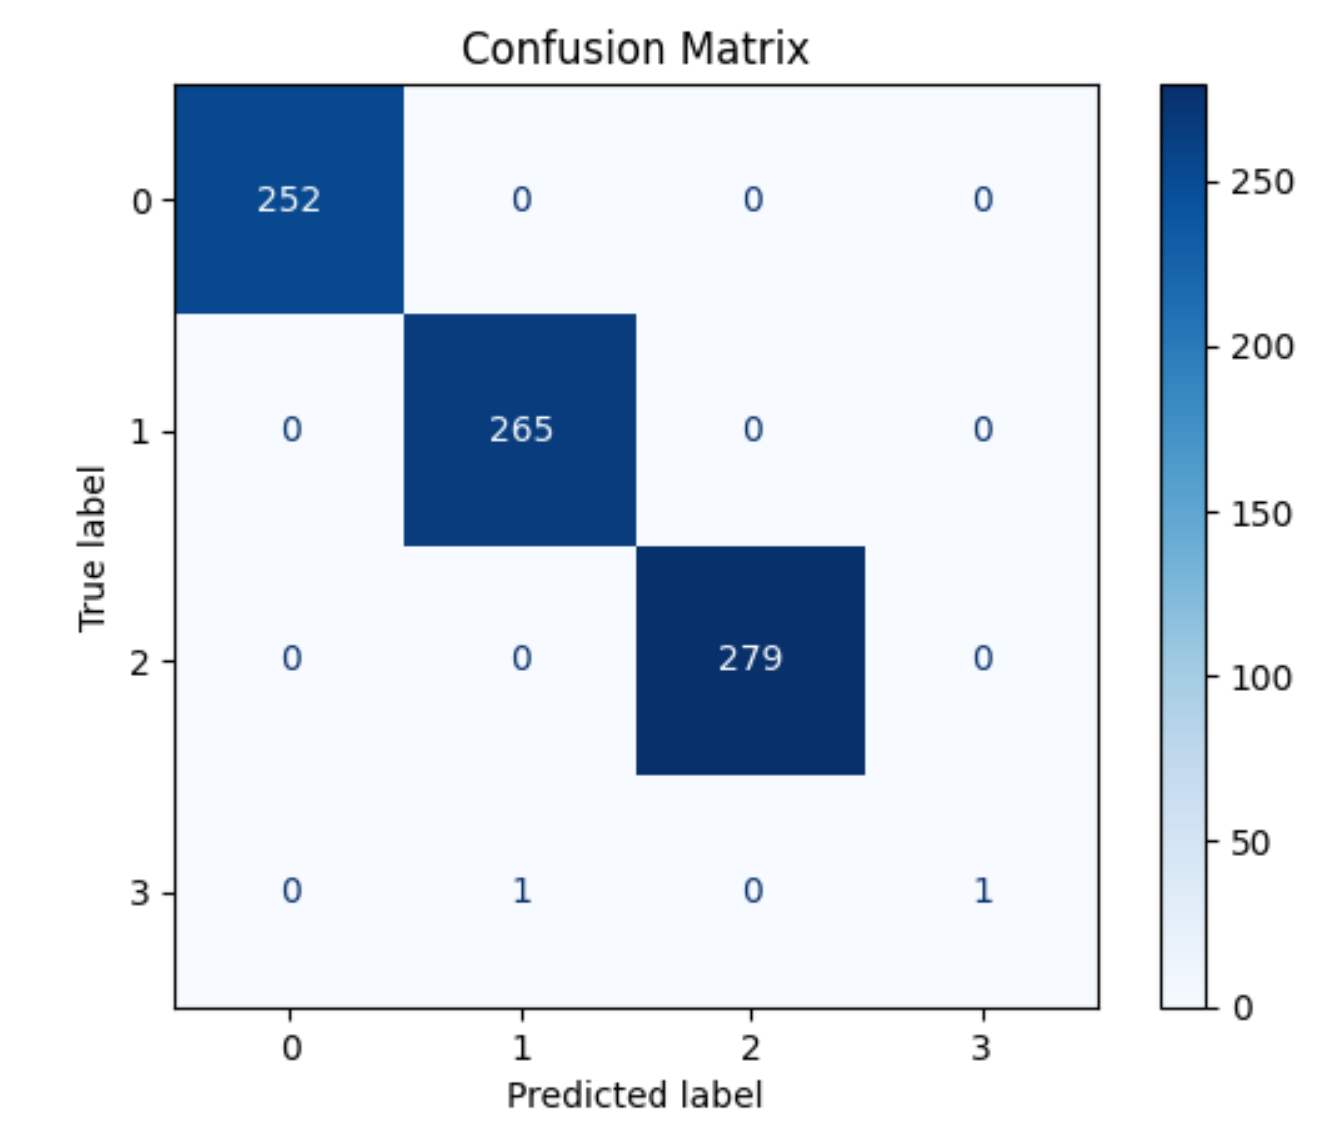
\includegraphics[width=\columnwidth]{svm_joint_expanded_WtoF.png}}
\caption{SVM Confusion Matrix for Joint Detection on Expanded Dataset With Wrist to Finger Distances}
\end{center}
\vskip -0.3in
\end{figure}

\subsection{Support Vector Machines for Joint Detection on Expanded Dataset with All Joints}
We also ran a similar SVM model with all joints instead of only the distances between the wrist and fingers. Our results are in Figure 7. We reached 92.2\% accuracy on the test set.

\begin{figure}[h]
\vskip -0.1in
\begin{center}
\centerline{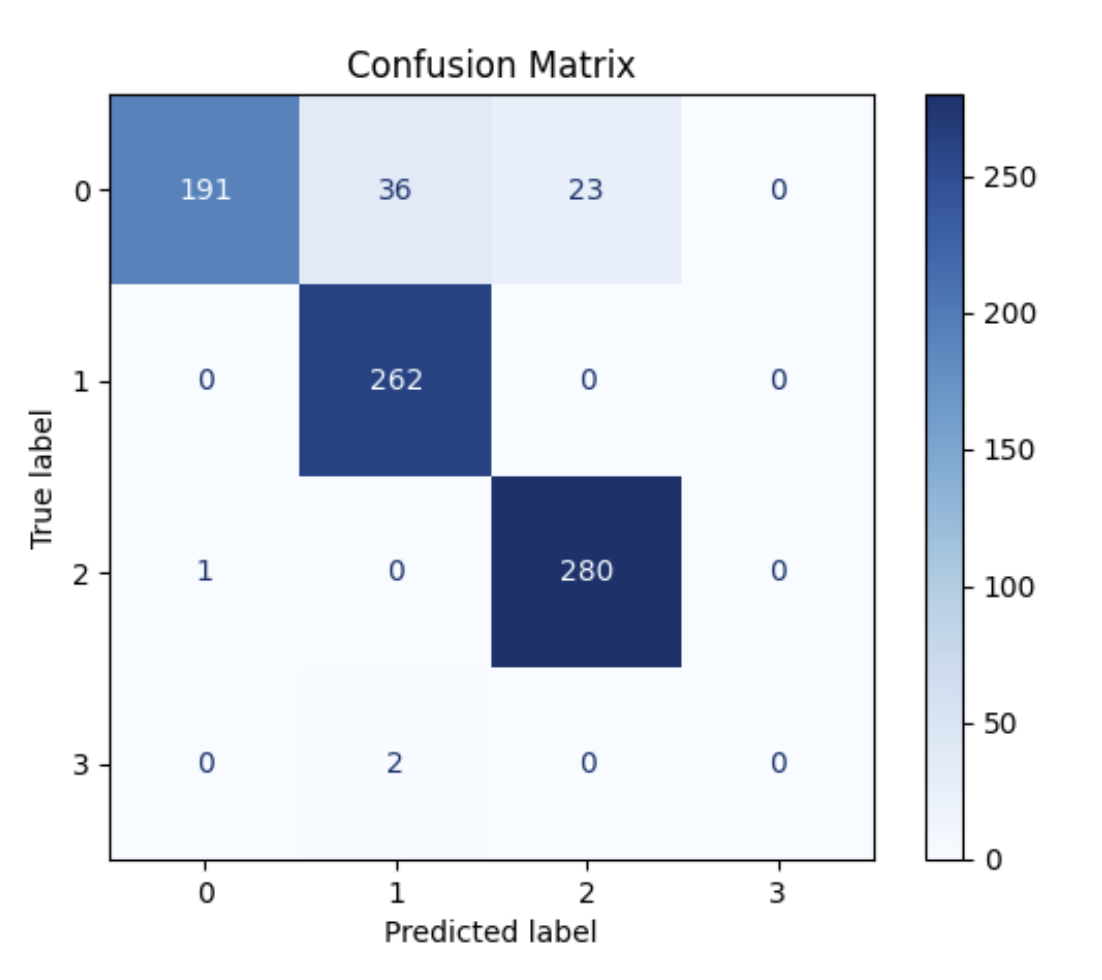
\includegraphics[width=\columnwidth]{svm_joint_expanded_all_joints.png}}
\caption{SVM Confusion Matrix for Joint Detection on Expanded Dataset With All Joints}
\end{center}
\vskip -0.3in
\end{figure}

\subsection{Game Playing Program}
We were able to successfully implement the game playing program with our specifications. A video of the demo can be seen at \url{https://www.youtube.com/watch?v=MK3ep_L7Mtc}. Though our underlying models had 100\% accuracy on the test set, the program is still subject to the following constraints. When no hand is in frame, the model never assigns joints and correctly never predicts a classification. The standard angle for our tests is palm facing the camera, fingers pointed up. At this angle, rock, paper, and scissors are all classified correctly when close to the camera, as long as the entire hand is in frame, which happens at 20 cm away from our camera. Moving away from the camera, rock is classified as paper when the hand is 75 cm from the camera, paper is classified as rock at 45 cm, and scissors is classified as paper at 48 cm. Rotating the hands such that the palm still faces the camera does not affect the classification or distances to breakdown at all since our model is only based on distances from the fingers to the wrist, not angle to wrist. Rotating the hands such that the side of the hands faces the camera, both at 45\textdegree and 90\textdegree angles, is subject to the same distance constraints as no rotation, so these rotations have no effect on the classification. Rotating the hands such that the fingers face the camera is subject to different distance constraints. At 45\textdegree, rock classifies as paper at 52 cm, paper classifies as rock at 25 cm, and scissors classifies as any of the three at 30 cm. At 90\textdegree, rock classifies as paper at 33 cm and both paper and scissors break completely, classifying as either rock or no classification at all distances. In total, our game playing program is very resilient to distance and rotations of the hand. As long as the fingers are not rotated to point towards the camera, maintaining that the fingers are perpendicular to the camera, all hand positions are correctly classified within 45 cm of the camera while still fully in the camera's frame. For our testing, we used a 720p HD Webcam with no zoom.

\section{Discussion and Conclusions}

\begin{table}[h]
\vskip -0.1in
\caption{Summary of Models}
\label{tab:nonjoint}
\centering
\small
\begin{tabular}{c | c | c}
\toprule
Model & Training Dataset & Accuracy \\
\midrule
SVM & Base (PCA) & 63.4\% \\
\midrule
CNN & Base (Direct) & 100\% \\
\midrule
CNN & Expanded (Direct) & 99.85\% \\
\midrule
ViT & Expanded (Direct) & 99.56\% \\
\midrule
SVM & Base (Joint) & 100\% \\
\midrule
NN & Base (Joint) & 100\% \\
\midrule
K-means & Base (Joint) & 80.2\% \\
\midrule
SVM & Expanded (with all joints) & 92.2\% \\
\midrule
SVM & Expanded (wrist to fingers) & 99.4\% \\
\midrule
K-means & Expanded (Joint) & 86.8\% \\
\bottomrule
\end{tabular}
\end{table}

Our image recognition models are summed up in Table 3. First, PCA saw limited success. Though SVMs proved useful in other contexts, the SVM for PCA on the Base dataset performed significantly worse than any other model despite over 99\% training accuracy. Although prior research does not explicitly explain why SVM models were not attempted, we believe that they did not attempt PCA with SVM because it produced much worse accuracy than the other models that they described \cite{CNNM} \cite{Ahmed2023RockPaperScissorsIC}. In addition, the previous study on sign language image recognition produced similar validation and training accuracy, so our results are relevant in this context \cite{Chowdary2023SignLR}. Our implementation of PCA is confirmed through successful reconstruction of the original image. Therefore, we hypothesize that although PCA is valuable in feature reduction, it is sensitive to backgrounds. Background color often affects a large number of features, and the Base training set had only white backgrounds. Therefore, PCA did not generalize to diverse background colors.
K-means clustering for both the Base and Expanded datasets on joint detection data produced better accuracy than SVM for PCA, but still much worse accuracy than other models. We believe that this is because the images are not simply separable like k-means clustering expects, so more complex models are needed to accurately explain the data. In addition, k-means clustering worked better on the Expanded dataset than the Base dataset. This could be due to the Kaggle dataset (in the Expanded but not Base dataset) having more separable data by k-means clustering than the Base dataset by itself.
Our CNN models produced very accurate results, up to 100\% accuracy on the Base dataset and 99.85\% accuracy on the Expanded dataset. Although past research has been done using the Kaggle dataset, over 99\% accuracy is consistent with the results from this previous research \cite{CNNM} \cite{Ahmed2023RockPaperScissorsIC}. Since the expanded dataset includes both the Kaggle dataset and other data, reaching similar accuracy to previous models with this Expanded dataset shows that we successfully made the models more robust.
For joint detection, our SVM and NN models on the Base dataset produced 100\% validation accuracy. Since these models run much more quickly than the SVM for PCA and CNN models on the Base dataset, joint detection did improve the accuracy with respect to efficiency of the models.
The SVM models on the Expanded dataset for joint detection were promising. Using only the wrist to finger distances, we reached 99.4\% accuracy, which is similar to previous research on the Kaggle dataset. Our hypothesis that only using wrist to finger distances would improve accuracy was correct, as our SVM improved by 7\% accuracy when using only these distances. Our model for SVM joint detection with wrist to finger distances for the Expanded dataset is the best model that we created, as it has fast training, works on the expanded dataset, and produces extremely high accuracy. Since our accuracy is similar to previous research, we successfully improved the robustness of previous models by including an Expanded dataset and joint detection.
Finally, implementing the game playing program was a success. We were able to build the program to accurately classify hand gestures in real time, subject to well-established constraints. In the future, to improve the accuracy when hands are far from the camera, we could experiment with better normalizing the distances between the wrist and the fingers in our calculations. That way, hands far from the camera do not default to low distances to the wrist. A similar program could be implemented with similar features for other hand gesture related tasks, such as sign language detection.
In addition to all of the models that we are implementing, many models have been attempted that we did not implement. For example, the You Only Look Once (YOLO) algorithm, an algorithm designed for general purpose object detection, has been attempted on rock paper scissors with a self made dataset, producing over 90\% accuracy with different versions of the model \cite{yolo}. For future work, we would suggest comparing our models with other machine learning models and pre-trained algorithms, such as the YOLO algorithm. In addition, although we attempted one Vision Transformer architecture, we could experiment with others. A ViT, OmniVec, currently has the best classification accuracy in the ImageNet-1k classification challenge \cite{imagenet}. However, Vision Transformers require more GPU power and data to achieve performance parity, so their usage remains an area of future study.

\section{Acknowledgements}
Marcus Kamen conducted Principal Components Analysis and k-means clustering models. Joseph Zou augmented the datasets with joint detection data and created the game playing demo. Galen Wei generated the expanded dataset and created the vision transformer and neural networks. Xutao Mao created the support vector machine models. \\
We thank Dr. Jonathan Sprinkle and for his assistance in the CS 4262/5262 course. We also thank Kuan-I (Gary) Chung for his assistance in the CS 4262/5262 course as well as his suggestion to incorporate joint detection into our project.

\section{Appendix}
Our code for our project can be found at \url{https://github.com/MarcusKamen/Image-Recognition-and-Joint-Detection-for-Rock-Paper-Scissors}. The preprocessing folder contains code for pushing our Expanded dataset to Hugging Face. All other files implement models either discussed in the paper or attempted but not discussed. We suggest uploading the code to Google Colab. However, the demo must be run on your local computer. Make sure to run "pip install" on all relevant imports to run the code, specifically "pip install gdown" and "pip install opencv-python."

\bibliography{main.bib}
\bibliographystyle{icml2021}

\end{document}
